% !TeX spellcheck = en_GB
\subsection{The automatic index updating feature}

As already stated in \ref{automatic_indexing_problematic_intro}, the automatic index updating feature is a must have for Hibernate Search GenericJPA. As this is arguably the most complicated feature for GenericJPA, we will go into detail about how we are achieving it next.

\subsubsection{Overview of possible implementations}

There are several approaches to building a automatic index updating feature. While they are all different in the specifics, they can generally be separated into two different categories: \textbf{synchronous} and \textbf{asynchronous}. Synchronous in this context means that the index is updated as soon as the newly changed data is persisted in the database without any real delay while in an asynchronous updating mechanism an arbitrary amount of time passes before the index is updated. While synchronous approaches are needed in some rare cases, fulltext search generally doesn't require a 100\% up-to-date index as a search index generally is not the source of truth in an application (only the database contains the "truth").
\\\\
We will now work out a solution for both sync and async needs, while the async version will serve as a backup whenever the synchronized mechanism is not applicable.

\paragraph{Synchronous approach}

\subparagraph{JPA events}

As we are trying to work with as little vendor specific APIs, JPA's callback events looks like a suitable candidate for listening to changes in entities.
\\\\
To listen for the JPA events we have two options: annotate the entities with callback methods or create a separate listener class. We will only take a look at the listener class as we don't want to have unnecessary methods in a possible user's entities. This class doesn't have to implement an interface, but has to have methods annotated with special annotations. The relevant ones are @PostPersist, @PostUpdate, @PostDelete (there are "pre-versions" available as well, but we focus on the post methods as they are more useful). What they stand for is quite self-explanatory.
\\\\
Such a class generally looks like this:
\\
\lstset{language=java}
\lstset{moredelim=[is][\bfseries]{[*}{*]}}
\begin{lstlisting}[frame=htrbl, caption={Example JPA entity listener}, label={lst:jpa_entity_listener.java}]
public class EntityListener {

	@PostPersist
	public void persist(Object entity) {
		//handle the event
	}
	
	@PostUpdate
	public void update(Object entity) {
		//handle the event
	}
	
	@PostDelete
	public void delete(Object entity) {
		//handle the event
	}

}
\end{lstlisting}
\noindent
It is then applied with an annotation on the entity:
\\
\lstset{language=java}
\lstset{moredelim=[is][\bfseries]{[*}{*]}}
\begin{lstlisting}[frame=htrbl, caption={Using a JPA entity listener}, label={lst:using_jpa_entitylisteners.java}]
[*@EntityListeners( { EntityListener.class } )*]
public class Book {

	//...

}
\end{lstlisting}
\noindent
As the JPA provider creates the EnityListeners automatically, we have no access to them without injecting a reference to them in a static way. While this might cause some Classloader problems, it should be fine in most cases.
\\
\lstset{language=java}
\lstset{moredelim=[is][\bfseries]{[*}{*]}}
\begin{lstlisting}[frame=htrbl, caption={Injecting the EntityListener}, label={lst:jpa_entity_listener.java}]
public class EntityListener {

	public EntityListener() {
		// inject it somewhere
		// so we can access it in a static way
		EntityListenerRegistry.inject(this);
	}

	//...

}
\end{lstlisting}

\noindent
Even though these listeners seem to be the perfect fit as they would enable us to fully integrate only with JPA interfaces, they have two big issues as we find out after investigating further.
\\\\
Firstly, not all JPA providers seem to handle these events similar, as for example Hibernate ORM doesn't propagate events from collection tables to the owning entity, while EclipseLink does (EclipseLink's behaviour would be needed from all providers).
\\\\
Secondly, we can see that the events are triggered on flush instead of commit. This is an issue if the changed data is not actually commited, but the index is updated:
\\

\lstset{language=java}
\lstset{moredelim=[is][\bfseries]{[*}{*]}}
\begin{lstlisting}[frame=htrbl, caption={Event triggering on flush}, label={lst:flush_event.java}]
EntityManager em = ...;

em.getTransaction().begin();

Book book = em.find( Book.class "someIsbn" );
book.setTitle( "someNewTitle" );

// flushes, so we retrieve the Book with the changes from above
// => event is triggered
List<Book> allBooks = 
	em.createQuery( "SELECT b FROM Book b" ).getResultList();

// we have no way to get this event to revert the wrong index change
em.getTransaction().rollback();
\end{lstlisting}

\noindent
While it \textbf{might} be possible to somehow fix the flush issue, the bad support from JPA providers like Hibernate ORM renders this approach unusable until the JPA providers work the same way to some reasonable extent.

\subparagraph{Native integration with JPA providers}

Almost every JPA provider has its own internal event system that is useful for cache invalidation and other relevant tasks. These combined with hooks into the transaction management allows us to build a proper index updating system that works with transactions in mind (big improvement compared to the flush() issues of plain JPA)
\\\\
By definition, these kind of integrations are not portable between JPA providers and require us to write different systems for all the JPA providers. But as the landscape for popular JPA providers probably only consists of Hibernate ORM, EclipseLink and OpenJPA, we can implement listeners for these and the others will have to rely on the async backup approach (as of the time of writing this, only Hibernate ORM and EclipseLink native integrations exist).
\\\\
As this seems to be the only reasonable solution for a synchronous update system, we will go with it in Hibernate Search GenericJPA.
\\\\
\textit{Note: we don't describe how these event systems are built in particular as they differ a lot in their APIs, but all are straightforward to use and describing the usage would be unspectacular.}

\paragraph{Asynchronous Trigger approach}
~\\



\subparagraph{Implementation details}

includeEmbeddedObjectId = true ist Pflicht!

\lstset{language=java}
\lstset{moredelim=[is][\bfseries]{[*}{*]}}
\begin{lstlisting}[frame=htrbl, caption={Book.java with Hibernate Search annotations}, label={lst:book.java_3}]
@Entity
@InIndex
@Table(name = "Book")
@Indexed
[*@UpdateInfo(
	tableName = "Book", 
	idInfos = 
	@IdInfo(columns = 
		@IdColumn(
			column = "isbn", 
			columnType = ColumnType.STRING
		)
	)
)*]
public class Book {

	// ... unchanged. 
	
	//mapping table events handled on Author side
	
	//getters & setters ...
}
\end{lstlisting}

\lstset{language=java}
\lstset{moredelim=[is][\bfseries]{[*}{*]}}
\begin{lstlisting}[frame=htrbl, caption={Author.java with Hibernate Search annotations}, label={lst:author.java_3}]
@Entity
@InIndex
@Table(name = "Author")
[*@UpdateInfo(
	tableName = "Author", 
	idInfos = 
	@IdInfo(columns = 
		@IdColumn(
			column = "authorId", 
			columnType = ColumnType.LONG
		)
	)
)*]
public class Author {
	
	// ... unchanged.
	
	[*@UpdateInfo(tableName = "Author_Book", 
		idInfos = {
		@IdInfo(entity = Author.class, 
			columns = 
			@IdColumn(
				column = "authorFk",
				columnType = ColumnType.LONG
			)
		),
		@IdInfo(entity = Book.class,
			columns = 
			@IdColumn(
				column = "bookFk",
				columnType = ColumnType.STRING
			)
		)
	})*]
	private Set<Book> books;
	
	//getters & setters ...
}
\end{lstlisting}

\begin{figure}[ht]
	\centering
	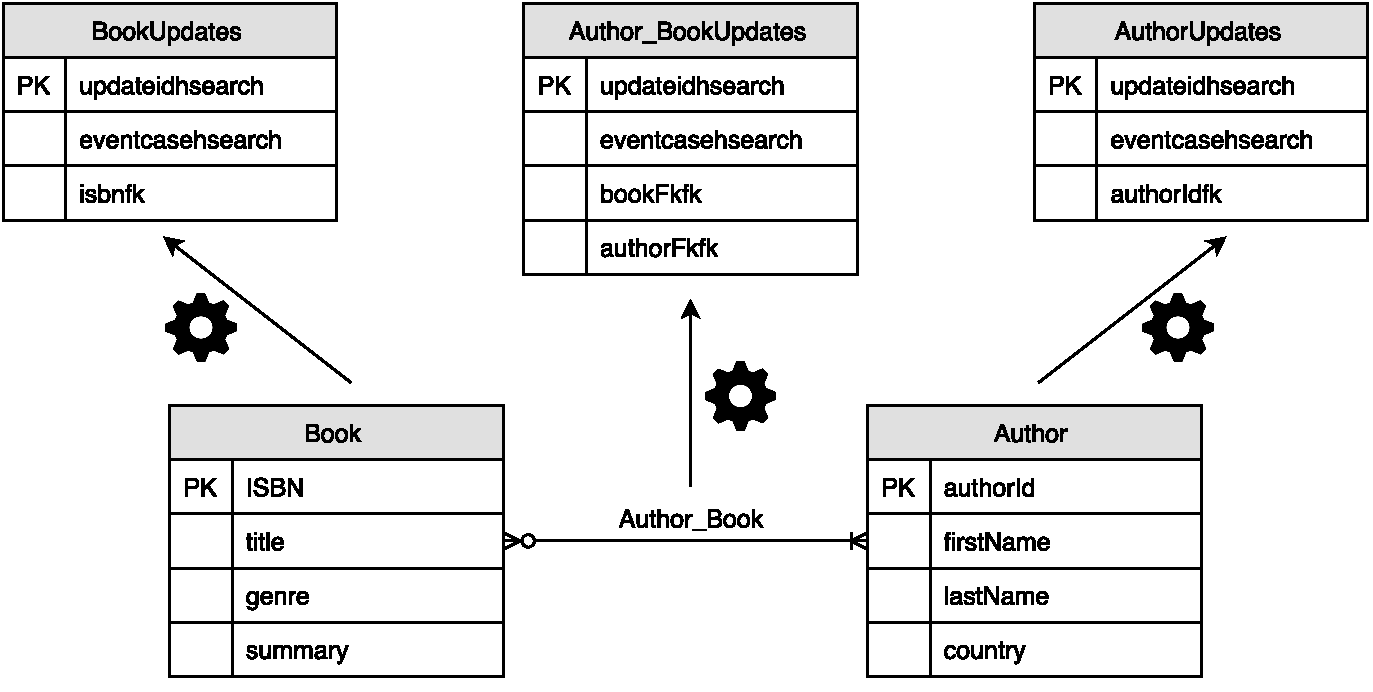
\includegraphics[scale=0.6]{images/Triggers_Schema.pdf}
	\caption{Triggers for the example project}
	\label{triggers_schema}
\end{figure}

\subsubsection{Complete Update System overview}

\begin{figure}[ht]
	\centering
	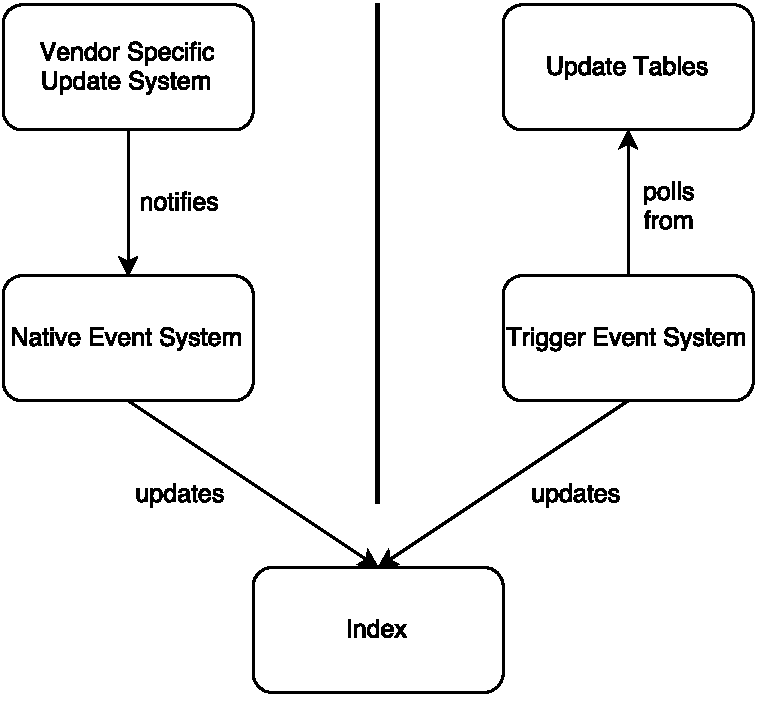
\includegraphics[scale=0.6]{images/UpdateConsumer_Architecture.pdf}
	\caption{Triggers for the example project}
	\label{updateconsumer_architecture}
\end{figure}

\pagebreak